% senior_thesis-proposal.tex
% Braden D. Licastro
% CMPSC 580, Spring 2013
%
% Oct 4, 2013
%
% This document provides a sample senior thesis proposal template for use
% by students in Allegheny's CS and Applied Computing programs.
%
%   *******************************************************************
%   * LOOK FOR BLOCK COMMENTS SUCH AS THIS ONE FOR AN EXPLANATION OF  *
%   * THIS DOCUMENT AND HOW TO MODIFY IT FOR YOUR OWN PROPOSAL!       *
%   *                                                                 *
%   * ANY LINE BEGINNING WITH A "%" IS A LATEX COMMENT AND IS IGNORED *
%   * BY THE LATEX PROCESSOR. YOU ARE ENCOURAGED TO COMMENT YOUR OWN  *
%   * LATEX CODE.                                                     *
%   *******************************************************************

%   ********************************************************************
%   * THE FIRST SECTION OF THE LATEX FILE IS THE "PREAMBLE." IT        *
%   * INSTRUCTS LATEX TO IMPORT SPECIAL PACKAGES FOR THINGS LIKE       *
%   * INCLUDING FIGURES, DOUBLE-SPACING, COLORED TEXT, ETC.            *
%   * DEPENDING ON YOUR NEEDS, YOU MAY FIND IT NECESSARY TO USE PACK-  *
%   * AGES THAT ARE NOT INCLUDED IN THIS TEMPLATE. SIMPLY IMITATE THE  *
%   * "\usepackage{...}" COMMANDS SHOWN BELOW.                         *
%   ********************************************************************

%   ********************************************************************
%   * BEGINNING OF PREAMBLE:                                           *
%   ********************************************************************
\documentclass[11pt]{article}

\usepackage[T1]{fontenc}
\usepackage{mathptmx}
\topmargin 0.0in
\setlength{\textwidth} {420pt}
\setlength{\textheight} {620pt} 
\setlength{\oddsidemargin} {20pt}
\setlength{\marginparwidth} {72in}
\setlength{\headheight}{14pt}

%   ********************************************************************
%   * Many of the commands below were simply copied over from an older *
%   * version of the proposal template; you can just leave them as     *
%   * they are (or you can delve into the TeX/LaTeX documentation      *
%   * and figure out what they do). Otherwise, jump ahead to the next  *
%   * block of comments, where you will enter title, abstract, etc.    *
%   ********************************************************************

\usepackage{fancyhdr} 
\usepackage{url}
\usepackage{graphicx}
\usepackage{epstopdf}
\epstopdfsetup{update} % only regenerate pdf files when eps file is newer

% set it so that subsubsections have numbers and they
% are displayed in the TOC (maybe hard to read, might want to disable)

\setcounter{secnumdepth}{3}
\setcounter{tocdepth}{3}

% define widow protection

\def\widow#1{\vskip #1\vbadness10000\penalty-200\vskip-#1}

\clubpenalty=10000  % Don't allow orphans
\widowpenalty=10000 % Don't allow widows

% this should give me the ability to use some math symbols that 
% were available by default in standard latex (i.e. \Box)

\usepackage{latexsym}

% define a little section heading that doesn't go with any number

\def\littlesection#1{
\widow{2cm}
\vskip 0.5cm
\noindent{\bf #1}
\vskip 0.0001cm 
}

\pagestyle{fancyplain}

\newcommand{\tstamp}{\today}   
\renewcommand{\sectionmark}[1]{\markright{#1}}
\lhead[\Section \thesection]            {\fancyplain{}{\rightmark}}
\chead[\fancyplain{}{}]                 {\fancyplain{}{}}
\rhead[\fancyplain{}{\rightmark}]       {\fancyplain{}{\thepage}}
\cfoot[\fancyplain{\thepage}{}]         {\fancyplain{\thepage}{}}

\newlength{\myVSpace}% the height of the box
\setlength{\myVSpace}{1ex}% the default, 
\newcommand\xstrut{\raisebox{-.5\myVSpace}% symmetric behaviour, 
  {\rule{0pt}{\myVSpace}}%
}

% leave things with no spacing extra spacing in the final version of the paper
\renewcommand{\baselinestretch}{1.0}    % must go before the begin of doc

% suppress the use of indentation for a paragraph

\setlength{\parindent}{0.0in}
\setlength{\parskip}{0.1in}

\begin{document}


% handle widows appropriately
\def\widow#1{\vskip #1\vbadness10000\penalty-200\vskip-#1}

% build the title section

\makeatletter

\def\maketitle{%
  %\null
  \thispagestyle{empty}%
  %\vfill
  \begin{center}%\leavevmode
    %\normalfont
    {\Huge \@title\par}%
    %\hrulefill\par
    {\normalsize \@author\par}%
    \vskip .4in
%    {\Large \@date\par}%
  \end{center}%
  %\vfill
  %\null
  %\cleardoublepage

  }

\makeatother

%   ********************************************************************
%   * Here is the first place where you need to begin customizing:     *
%   * Enter you name, the title of your proposal, etc., in the places  *
%   * indicated by the comment "% CHANGE!".                            *
%   ********************************************************************

\vspace*{-1.1in}
\title{Approximate Algorithmic Image Matching to Reduce Online Storage Overhead of User Submitted Images}  % CHANGE!

% build the author section
\author{
        Braden D. Licastro\\  % CHANGE!
        Department of Computer Science\\
        Allegheny College \\
        {\tt licastb@allegheny.edu}  \\  % CHANGE!
        \url{http://skynetgds.no-ip.biz/srthesis} \\   % CHANGE!
        \vspace*{.1in} \today \\ \vspace*{.1in}
}

\maketitle       % use the default title stuff

% Default "abstract" environment is too small; customize one instead:
\begin{center}
\large\bf Abstract
\vspace{-1em}  % Reduce space between header and the abstract
\end{center}

%   ********************************************************************
%   * Here is the second place where you need to customize:            *
%   * enter your abstract in the "quote" environment:                 *
%   ********************************************************************

\begin{quote}
Websites similar to Photobucket and imgur must be able to store massively increasing quantities of data; most of these sites already implement systems that limit the number, size, type of image, and compress the uploaded images to save space. Though these systems can be paired with file expiration times in which an upload is deleted, the cost of storage and backups of this data can be high. To further address this problem, the research aims to create an intelligent image uploading system capable of identifying near-duplicate image uploads on-the-fly; This system also provides the user with a higher resolution copy of their image from the server if available, thus providing better user experience while reducing unnecessary redundancy. By using the proposed system, the user will benefit from improved quality and service while the business can reduce storage and other various costs.
\end{quote}

%\vspace*{-.4in}
\section{Introduction}
\label{sec:introduction}
\vspace*{-.1in}

%   ********************************************************************
%   * Enter the text of your introductory section here.                *
%   ********************************************************************

Computers are absolutely everywhere, and society is becoming more digitized every day creating
a need for storage of large amount of files. When running a website, storage space is at a
premium, and the physical disks in the servers being used may not be local, but may in fact be
located around the world. By allowing user submitted data, it quickly becomes apparent that data
redundancy reduction can save a significant amount of storage space. This research will target
the problem of data redundancy and provide a solution that will reduce not only storage costs but
also inefficiencies. An implementation of a file management system will be introduced that is
capable of managing large volumes of files using a database of location pointers and hash keys
that identify each individual file. By using pointers, it is possible for the files to be stored on one
central location or distributed across several systems while avoiding long search times.
By using text based entries in a database, a hashing function can be implemented which is capable
of producing a unique hash code for each file in the collection. Because this key is unique for each
different file, it is a reliable gauge of uniqueness. When multiple files are found to be identical
only one physical copy will be kept but pointers to the database entry will allow easy access.
On large, distributed network storage servers, the benefits become ever more apparent. As users
store files on the disks, the system will hash each file and search for a match in a database,
thus allowing the user access to the data, but eliminating the overhead of storing numerous
copies of identical data. An increase in computation time will exist but should be minimal as
text comparisons will be the primary task in finding uniqueness, but this will be outweighed by
minimized physical storage requirements and costs of data backup.
The implementation of this system could be used in tandem with other currently implemented
methods of file space cost reduction technologies out of the box. By not only using the proposed
method of space requirement reduction, it could in theory be possible that with data expiration times, file size maximums, and similar technologies, that storage needs will plateau after the
initial surge of additions and the expiration time has passed for the earliest uploaded file. This
would allow webmasters to better predict overall needs and better predict upload trends and react
accordingly with preventative maintenance and any required space additions.

\vspace*{-.1in}
\section{Related Work}
\label{sec:relatedwork}
\vspace*{-.1in}

%   ********************************************************************
%   * Enter the text of your related work section here.                *
%   ********************************************************************

Summarize the previously published papers and books that are related
to your proposed research.  Whenever possible, you should compare and
contrast your approach with the ones that have been discussed in the
past.  As you describe your papers, please make sure that you cite
them properly.
\\Let's use the rest of this section to generate out bibliography!
\cite{nettuts:pdosqli}
\cite{about:rename}
\cite{php:uploads}
\cite{catpa:gdcode}
\cite{ubuntu:lampsetup}
\cite{nix:gdsetup}
\cite{php:gdimg}
\cite{Foo:2007}
\cite{Srinivasan:2008}
\cite{Lee:2010}.

\vspace*{-.2in}
\section{Method of Approach}
\label{sec:method}
\vspace*{-.1in}

%   ********************************************************************
%   * Enter the text of your method of approach section here.          *
%   ********************************************************************

Use technical diagrams, equations, algorithms, and paragraphs of text
to describe the research that you intend to complete. See the \LaTeX\ source
file for the proposal to learn how Figure \ref{intro-fig1} and Table 
\ref{intro-tab1} were included. Be sure to number all figures and tables and to
explicitly refer to them in your text.

\begin{figure}[htbp]
\centering
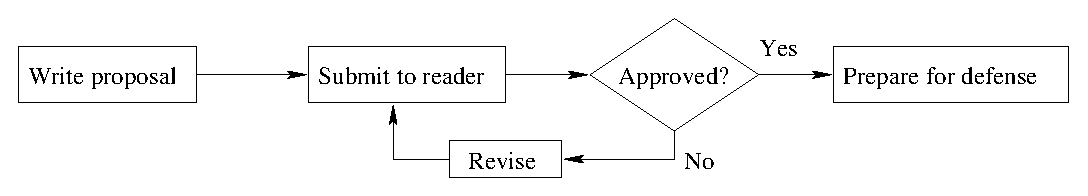
\includegraphics[width=5in]{flow}
\caption{Flow graph for proposal-writing}
\label{intro-fig1}
\end{figure}

\begin{table}[htbp]
\centering
\begin{tabular}{|c||c|c|}
\hline
\bf Task & \bf Begin Date & \bf End Date\\\hline\hline
First draft & Now & 20 Sept\\\hline
Second draft & 20 Sept & 27 Sept\\\hline
Third draft & 27 Sept & 4 Oct\\\hline
Fourth draft & 4 Oct & 11 Oct\\\hline
Fifth draft & 11 Oct & 18 Oct\\\hline
\end{tabular}
\caption{Proposed work schedule}
\label{intro-tab1}
\end{table}

\vspace*{-.2in}
\section{Evaluation Strategy}
\label{sec:evaluate}
\vspace*{-.1in}

%   ********************************************************************
%   * Enter the text of your evaluation strategy section here.         *
%   ********************************************************************

Explain what steps you will take to evaluate your proposed method.  If
you intend to conduct experiments, then you must clearly define your
evaluation metrics.

\vspace*{-.1in}
\section{Research Schedule}
\label{sec:schedule}
\vspace*{-.1in}

Identify the main phases and tasks of your research project and set
deadlines for when you will be able to complete each of these items.

\vspace*{-.1in}
\section{Conclusion}
\label{sec:conclusion}
\vspace*{-.1in}

%   ********************************************************************
%   * Enter the text of your concluding section section here.          *
%   ********************************************************************

Provide a summary of your proposed research and suggest the impact
that it may have on the discipline of computer science.  If possible,
you may also suggest some areas for future research.

\bibliographystyle{plain}
\bibliography{senior_thesis_proposal}

\end{document}

